% 本文件由 paper/generate-content.js 从游戏数据自动生成，请勿手工编辑。

\subsubsection{赵敏人物图录}

\Needspace{0.72\textheight}
\begin{figure}[H]
  \centering
  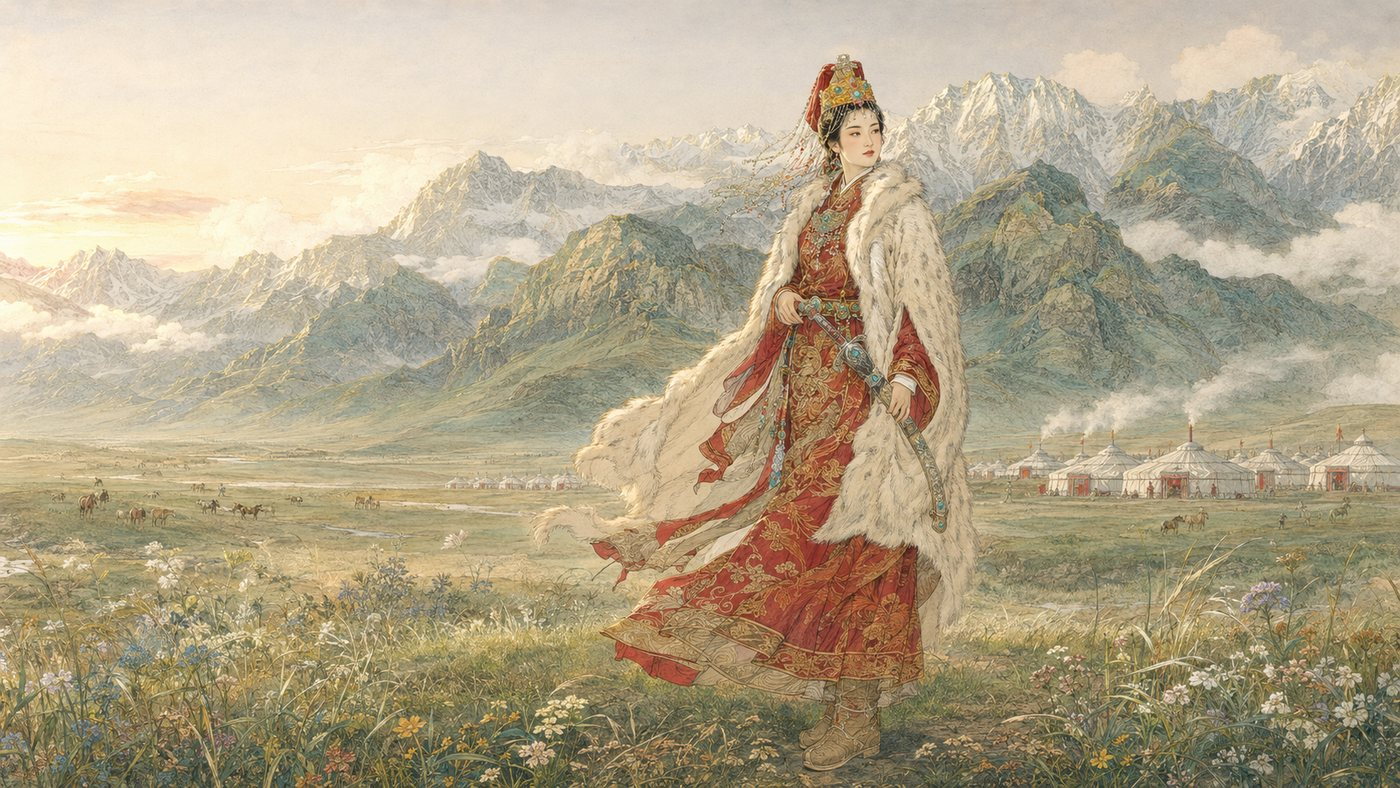
\includegraphics[width=0.92\linewidth,height=0.62\textheight,keepaspectratio]{assets/characters/zhaomin/portrait_01.jpg}
  \caption{赵敏第1拍《绿柳初逢》人物图。绿柳初逢。春柳、白貂与含而不露的笑意共同确立人物的机敏；冷白衣色与新绿背景相互映照，形成初见时的清锐感。}
  \label{fig:portrait:zhaomin:1}
\end{figure}

\Needspace{0.72\textheight}
\begin{figure}[H]
  \centering
  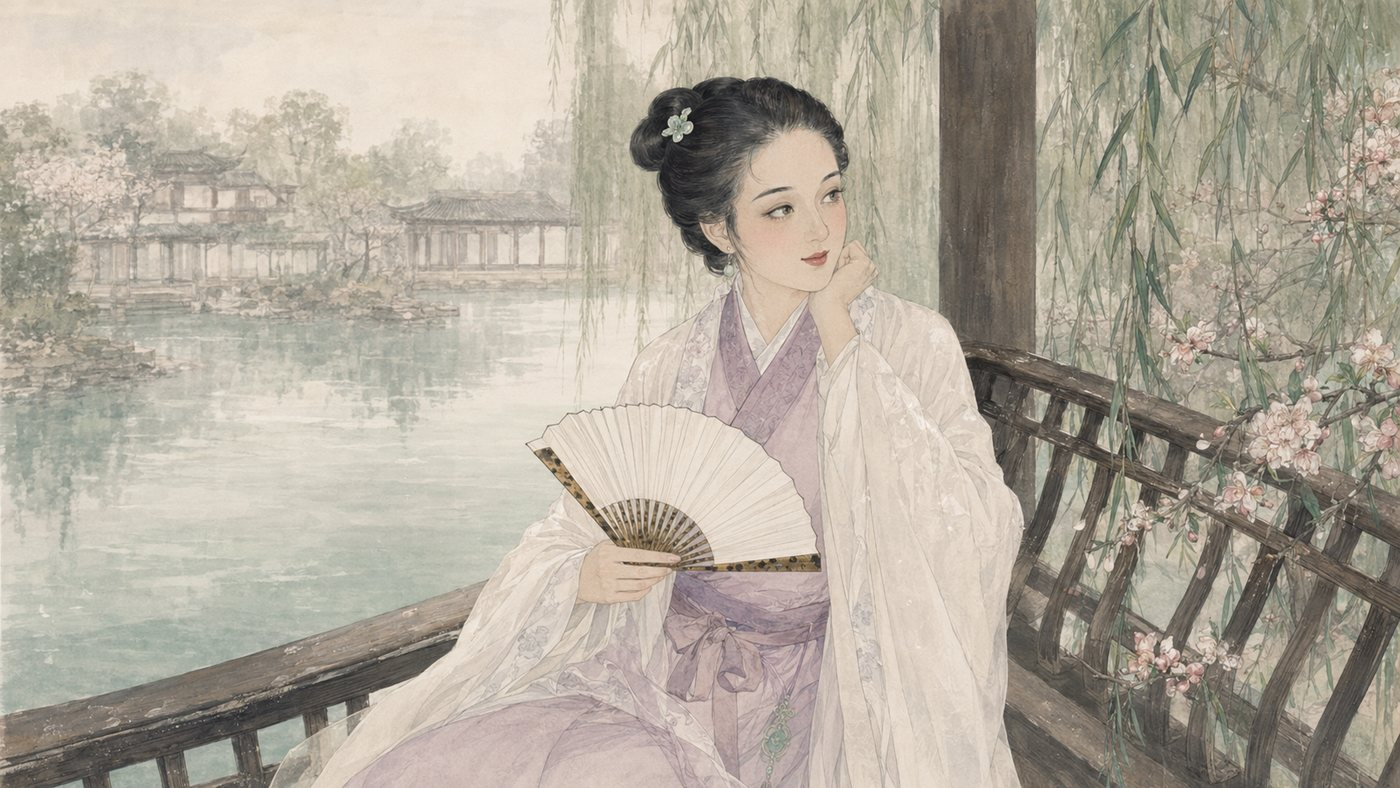
\includegraphics[width=0.92\linewidth,height=0.62\textheight,keepaspectratio]{assets/characters/zhaomin/portrait_02.jpg}
  \caption{赵敏第2拍《黑玉断续》人物图。黑玉断续。药物与伤体被置于同一视域，修复既是医理线索，也是关系重新建立的隐喻；暗色背景使人物的判断力成为视觉中心。}
  \label{fig:portrait:zhaomin:2}
\end{figure}

\Needspace{0.72\textheight}
\begin{figure}[H]
  \centering
  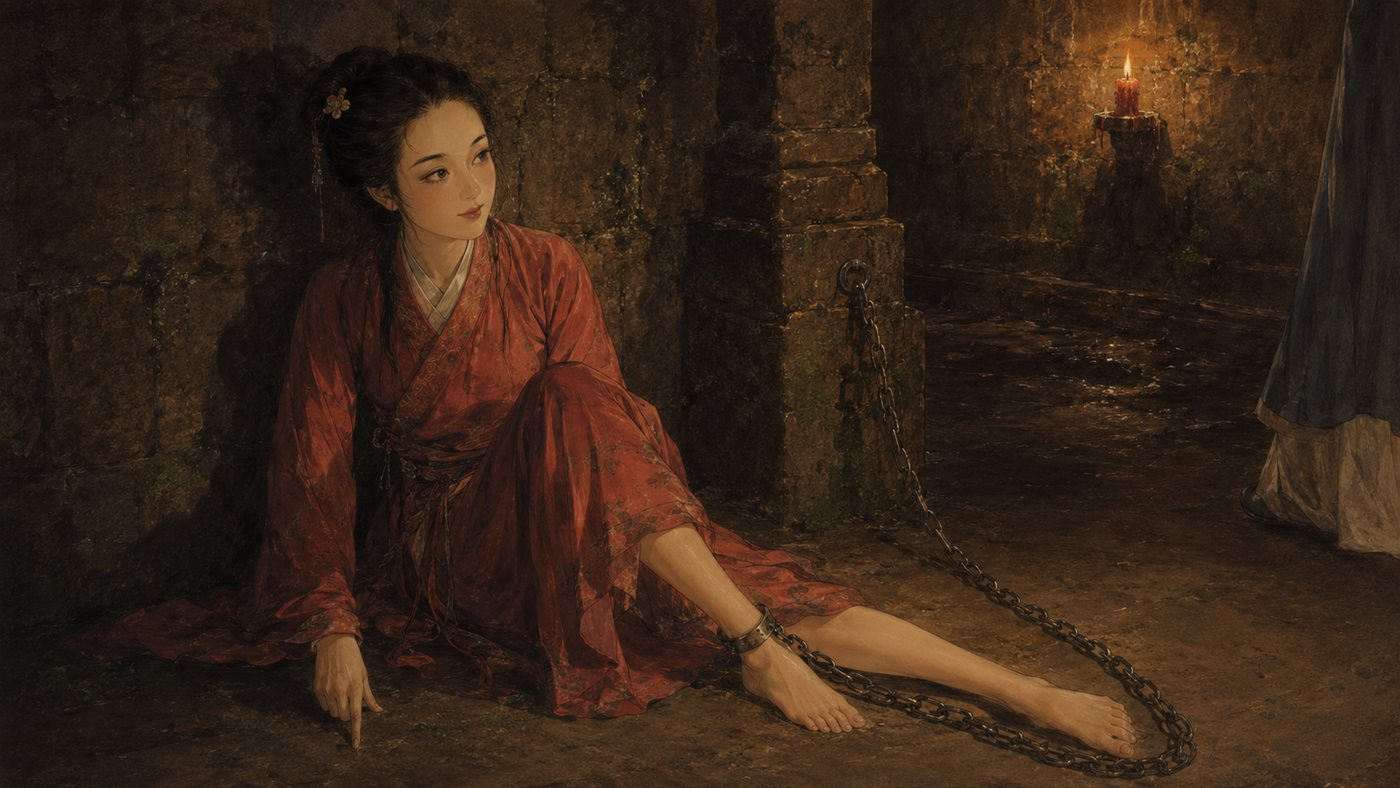
\includegraphics[width=0.92\linewidth,height=0.62\textheight,keepaspectratio]{assets/characters/zhaomin/portrait_03.jpg}
  \caption{赵敏第3拍《万安寺火》人物图。万安寺火。火光映照出危局中的决断，人物不以柔弱姿态出现；暖红与墨黑的强烈对照强化行动伦理与救援主题。}
  \label{fig:portrait:zhaomin:3}
\end{figure}

\Needspace{0.72\textheight}
\begin{figure}[H]
  \centering
  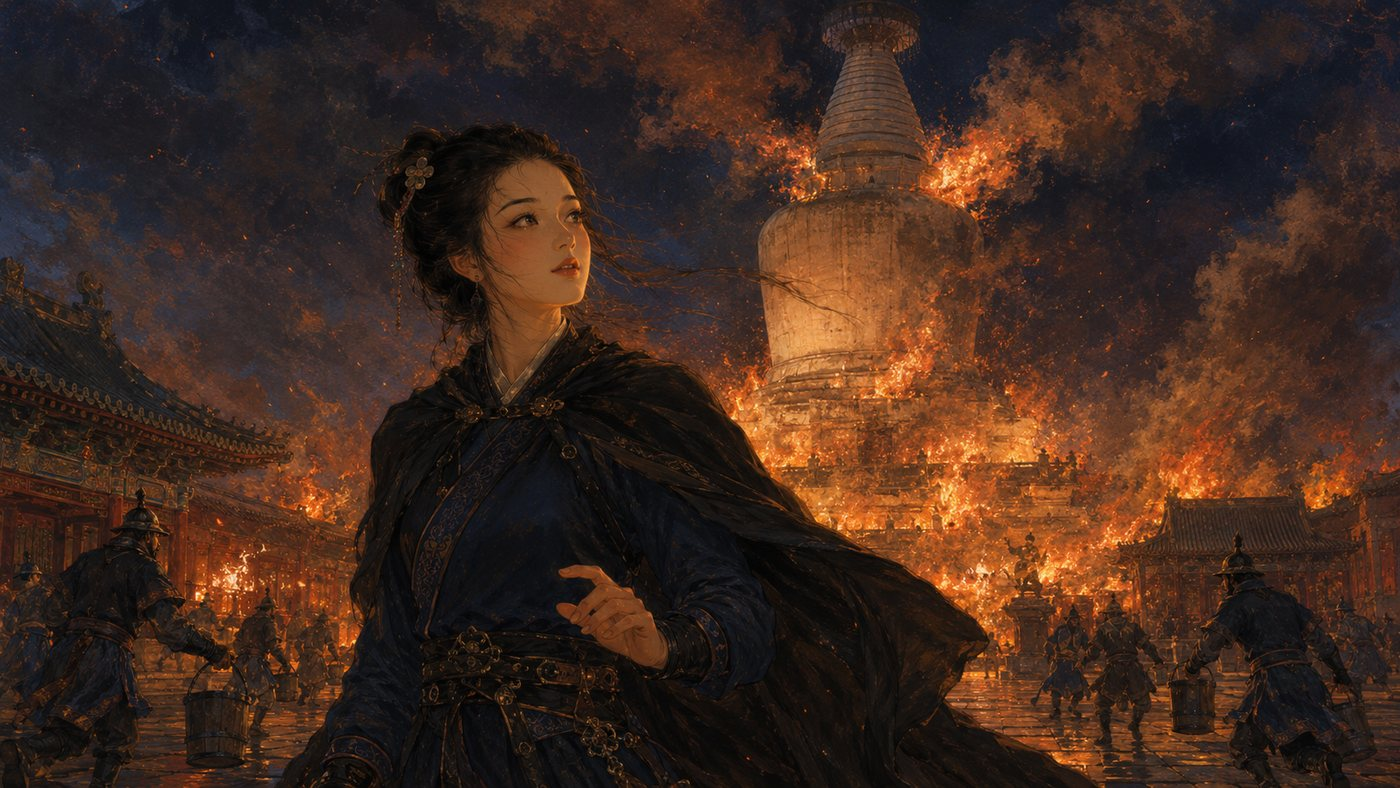
\includegraphics[width=0.92\linewidth,height=0.62\textheight,keepaspectratio]{assets/characters/zhaomin/portrait_04.jpg}
  \caption{赵敏第4拍《灵蛇海上》人物图。灵蛇海上。海雾、孤舟与远望构成漂泊感，暗示身份边界的松动；开阔留白使人物从权力中心暂时退入天地尺度。}
  \label{fig:portrait:zhaomin:4}
\end{figure}

\Needspace{0.72\textheight}
\begin{figure}[H]
  \centering
  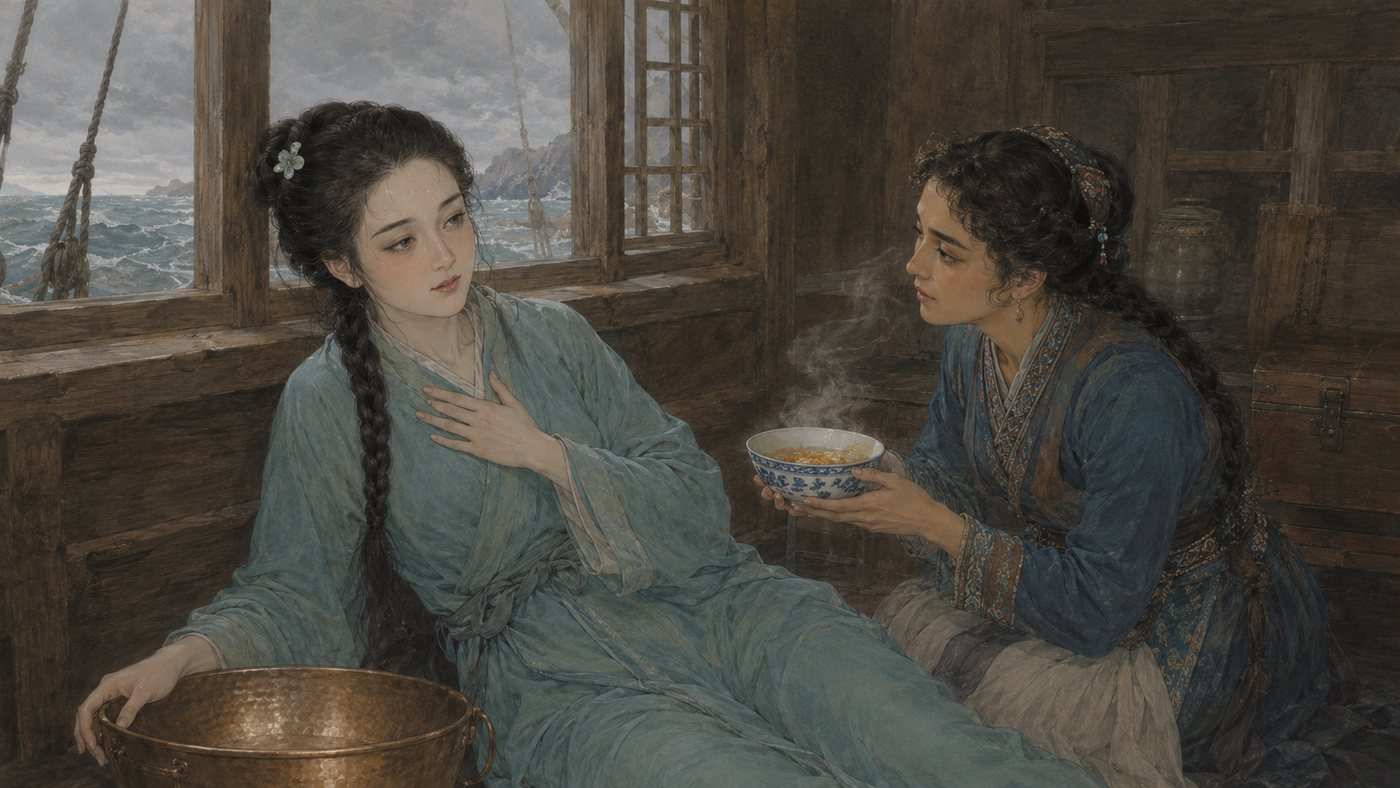
\includegraphics[width=0.92\linewidth,height=0.62\textheight,keepaspectratio]{assets/characters/zhaomin/portrait_05.jpg}
  \caption{赵敏第5拍《弥勒佛庙》人物图。弥勒佛庙。封闭建筑与斜入天光形成审问式空间，表现智谋背后的风险；构图以明暗分界提示真相并非全然可见。}
  \label{fig:portrait:zhaomin:5}
\end{figure}

\Needspace{0.72\textheight}
\begin{figure}[H]
  \centering
  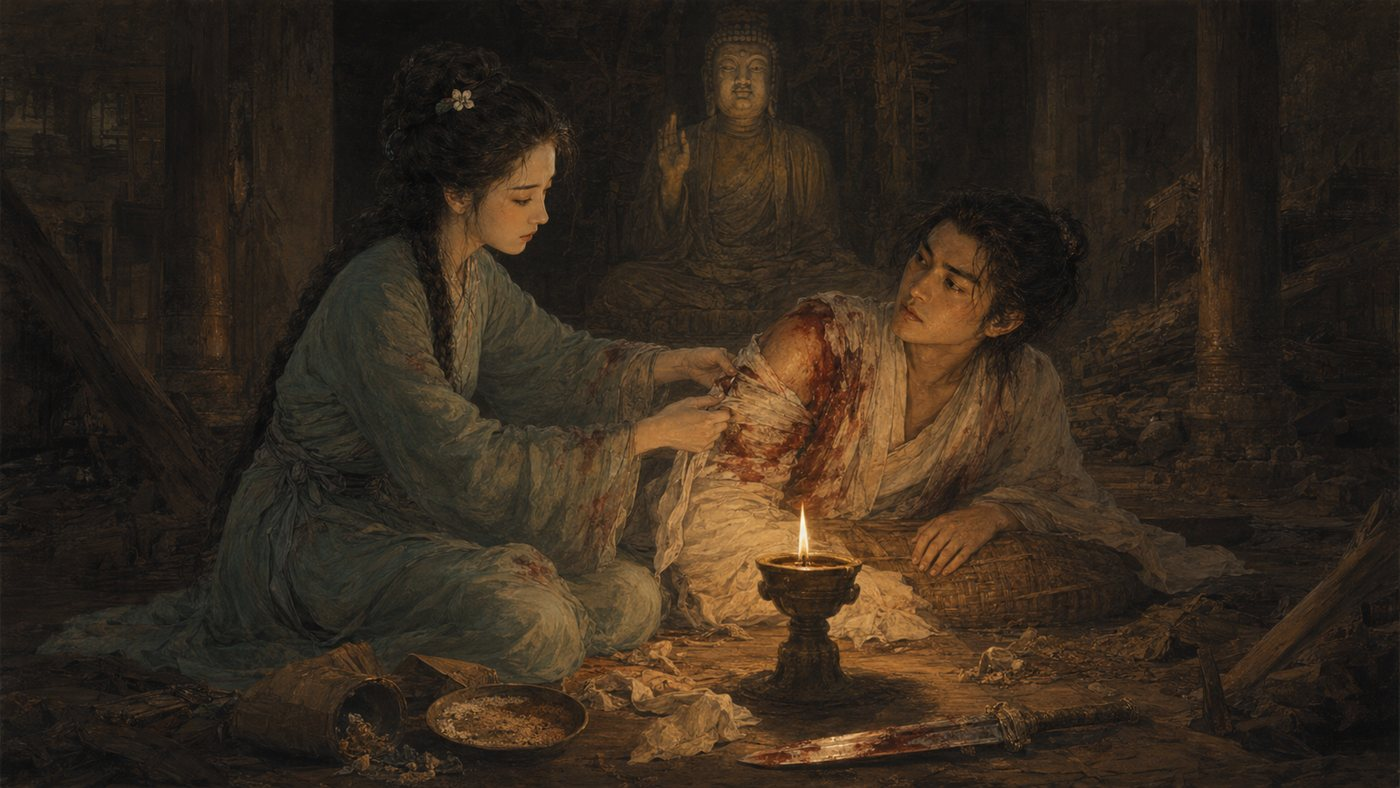
\includegraphics[width=0.92\linewidth,height=0.62\textheight,keepaspectratio]{assets/characters/zhaomin/portrait_06.jpg}
  \caption{赵敏第6拍《濠州夺婚》人物图。濠州夺婚。红色礼制空间被人物的侧身动作打破，象征个人选择对既定秩序的冲撞；高饱和朱红集中呈现情感张力。}
  \label{fig:portrait:zhaomin:6}
\end{figure}

\Needspace{0.72\textheight}
\begin{figure}[H]
  \centering
  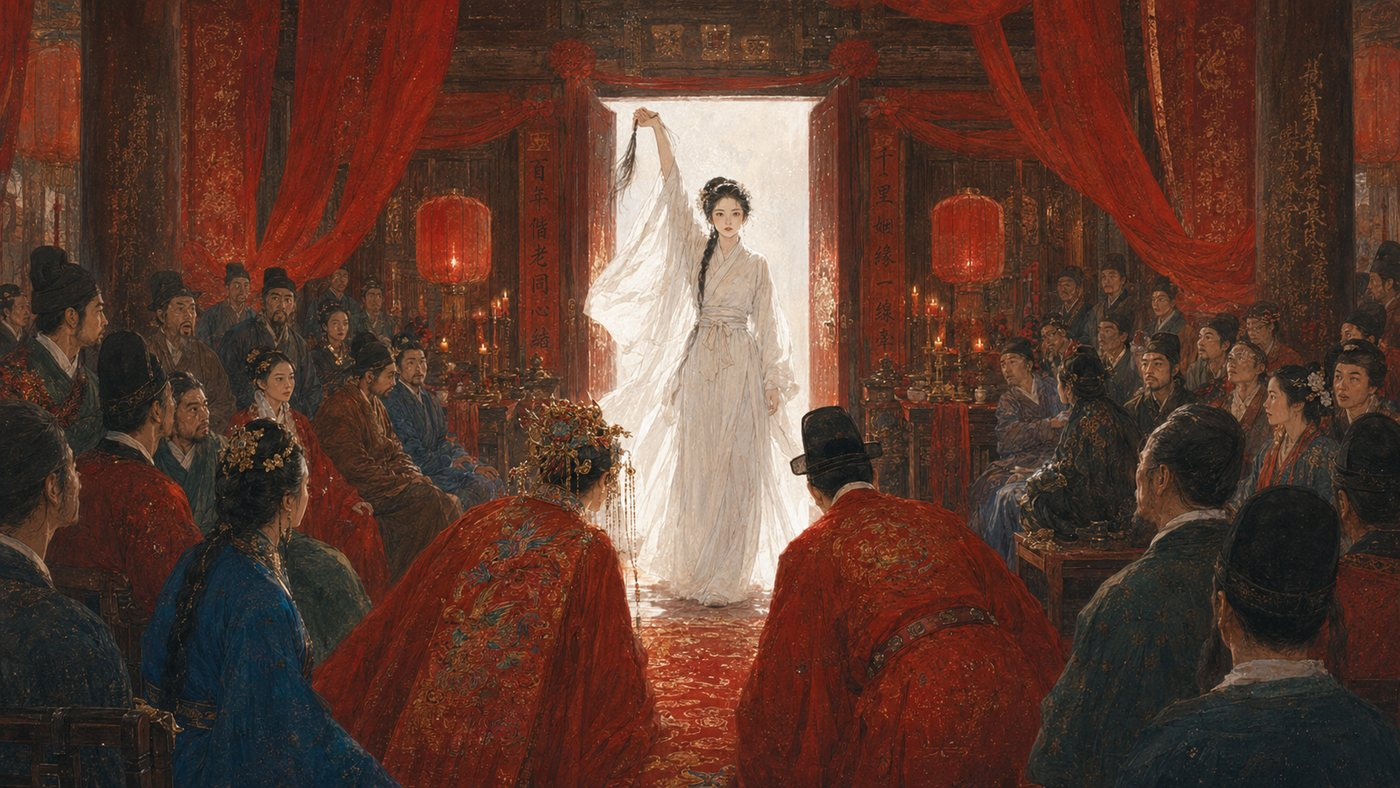
\includegraphics[width=0.92\linewidth,height=0.62\textheight,keepaspectratio]{assets/characters/zhaomin/portrait_07.jpg}
  \caption{赵敏第7拍《少室山下》人物图。少室山下。山门与石阶强调制度和传统的重量，人物的稳定站姿则保留自主意志；纵深透视使选择具有路径感。}
  \label{fig:portrait:zhaomin:7}
\end{figure}

\Needspace{0.72\textheight}
\begin{figure}[H]
  \centering
  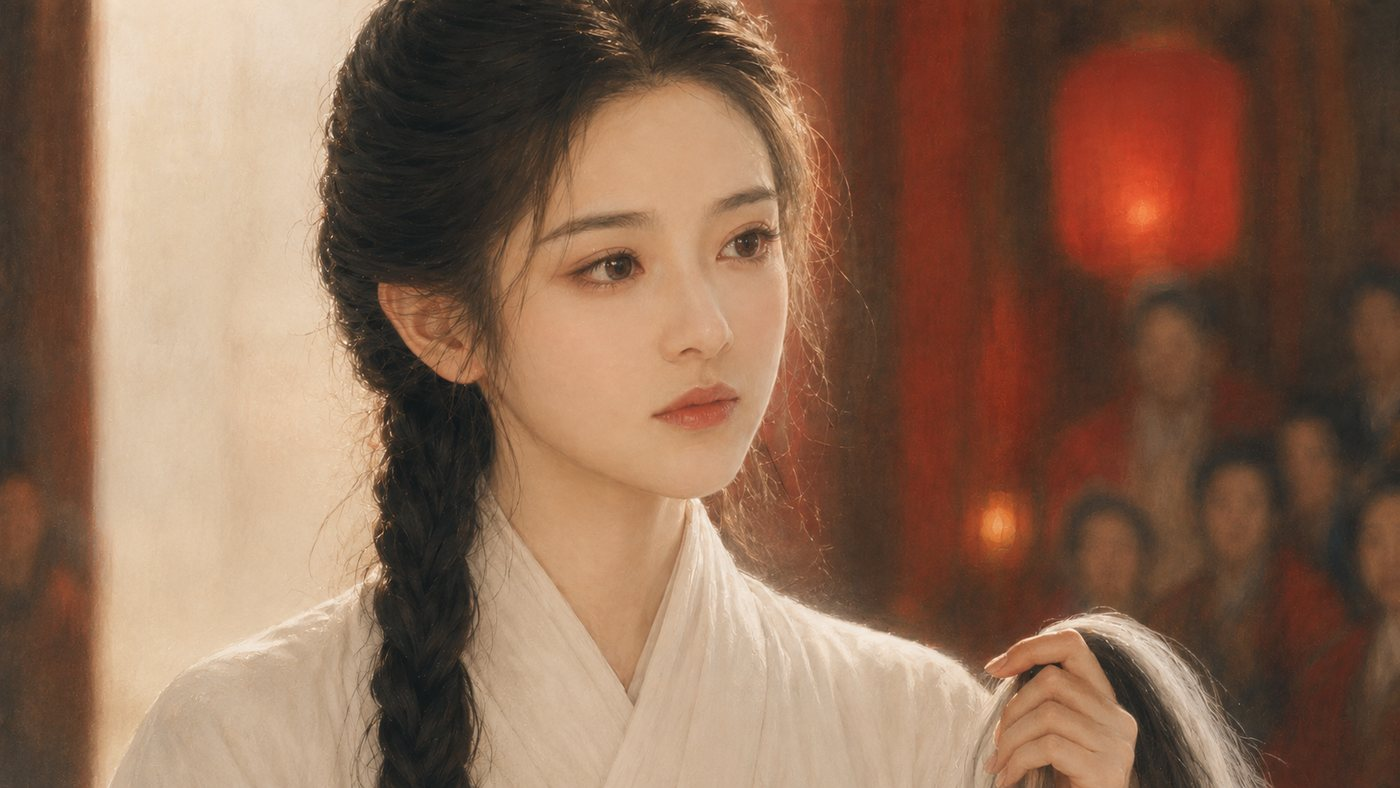
\includegraphics[width=0.92\linewidth,height=0.62\textheight,keepaspectratio]{assets/characters/zhaomin/portrait_08.jpg}
  \caption{赵敏第8拍《朔漠风霜》人物图。朔漠风霜。风沙削弱华饰，凸显身体对环境的真实承受；赭石与灰蓝构成冷暖错位，表现坚韧并非没有代价。}
  \label{fig:portrait:zhaomin:8}
\end{figure}

\Needspace{0.72\textheight}
\begin{figure}[H]
  \centering
  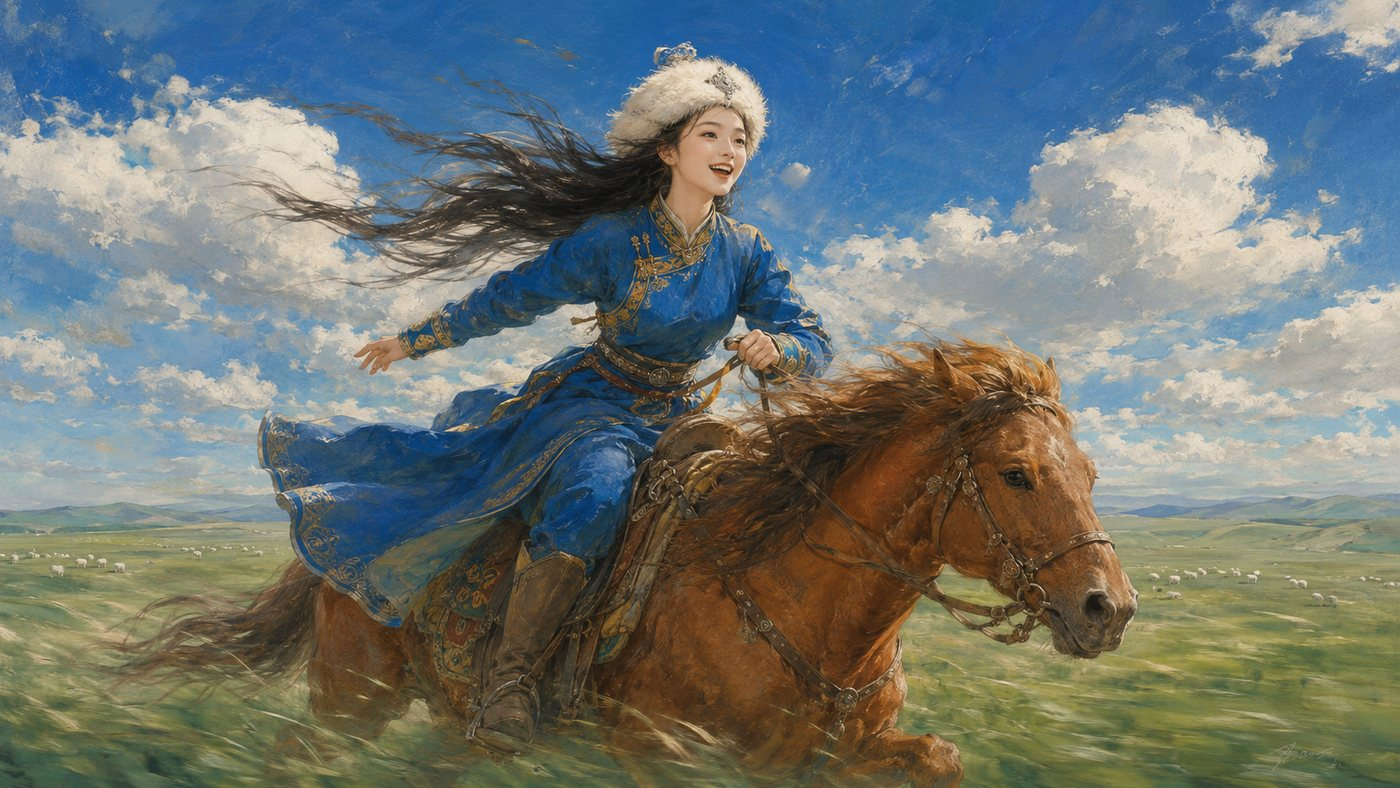
\includegraphics[width=0.92\linewidth,height=0.62\textheight,keepaspectratio]{assets/characters/zhaomin/portrait_09.jpg}
  \caption{赵敏第9拍《冰火之岛》人物图。冰火之岛。极寒与火山并置，象征生命处境中的冲突和调和；人物位于两种光源之间，成为平衡而非征服自然的主体。}
  \label{fig:portrait:zhaomin:9}
\end{figure}

\Needspace{0.72\textheight}
\begin{figure}[H]
  \centering
  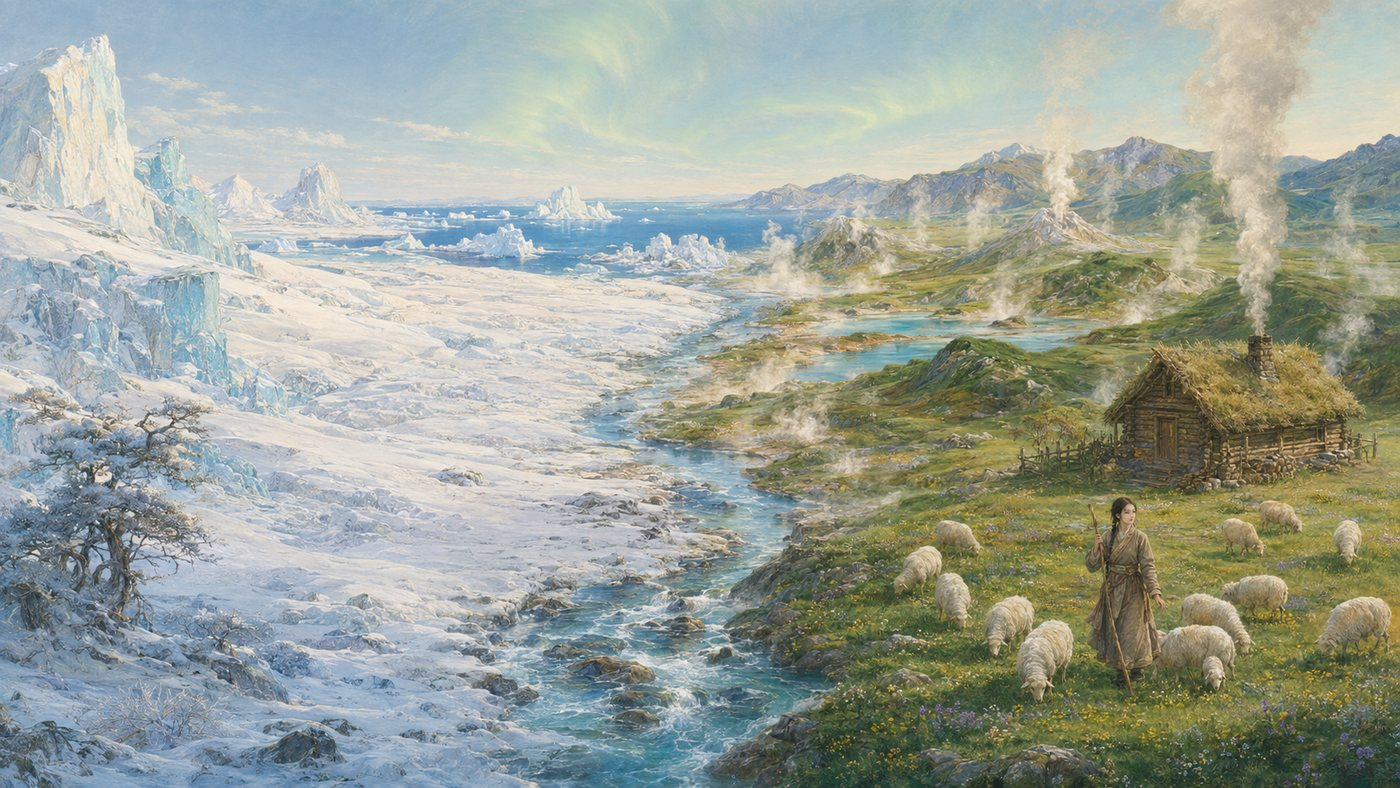
\includegraphics[width=0.92\linewidth,height=0.62\textheight,keepaspectratio]{assets/characters/zhaomin/portrait_10.jpg}
  \caption{赵敏第10拍《父女恩仇》人物图。父女恩仇。宫廷秩序与亲缘裂隙同时进入画面，人物表情克制，避免将伦理冲突处理为单一善恶；对称构图有意制造压迫感。}
  \label{fig:portrait:zhaomin:10}
\end{figure}

\Needspace{0.72\textheight}
\begin{figure}[H]
  \centering
  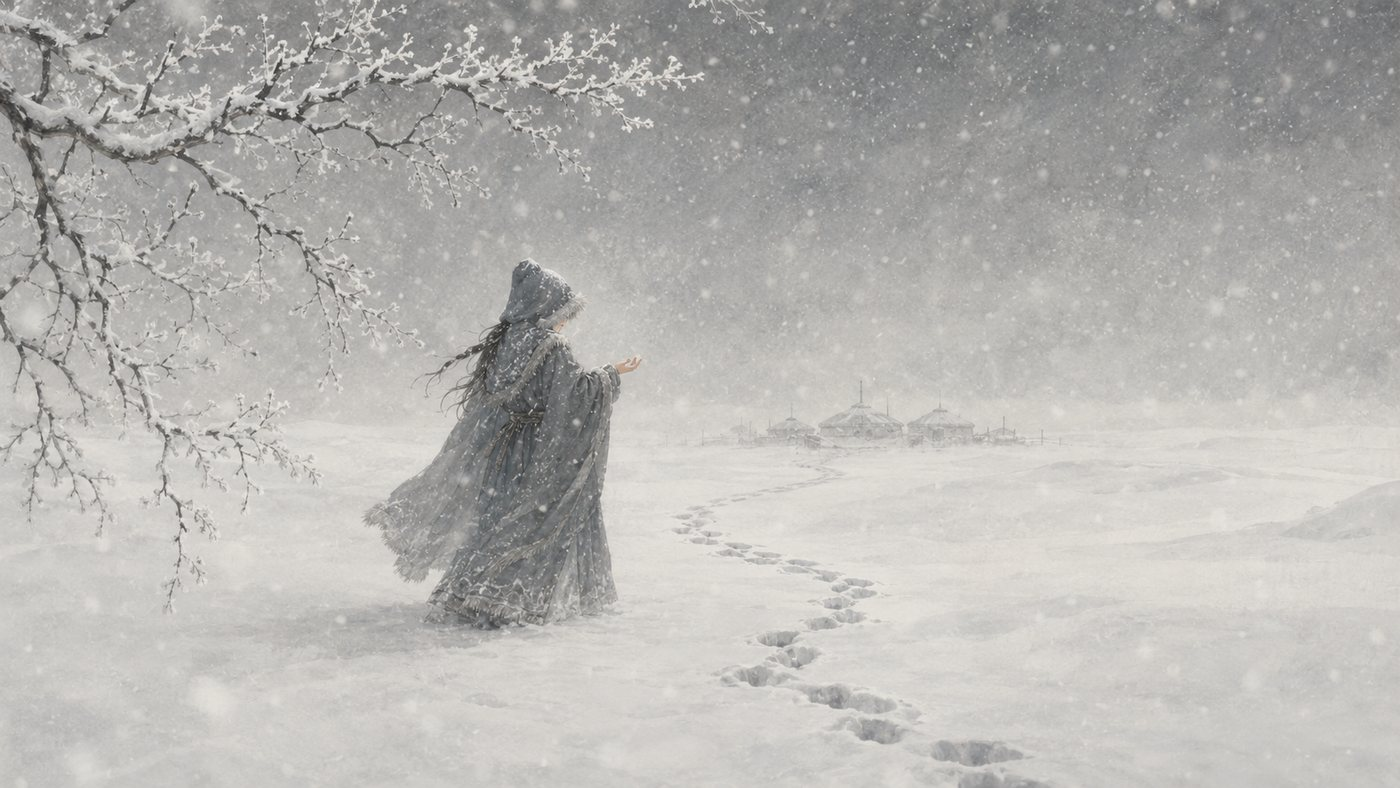
\includegraphics[width=0.92\linewidth,height=0.62\textheight,keepaspectratio]{assets/characters/zhaomin/portrait_11.jpg}
  \caption{赵敏第11拍《玄冥寒掌》人物图。玄冥寒掌。冷色侵入肤色，提示疾病与创伤首先发生于身体；局部暖光保留康复可能，使痛苦不被审美化。}
  \label{fig:portrait:zhaomin:11}
\end{figure}

\Needspace{0.72\textheight}
\begin{figure}[H]
  \centering
  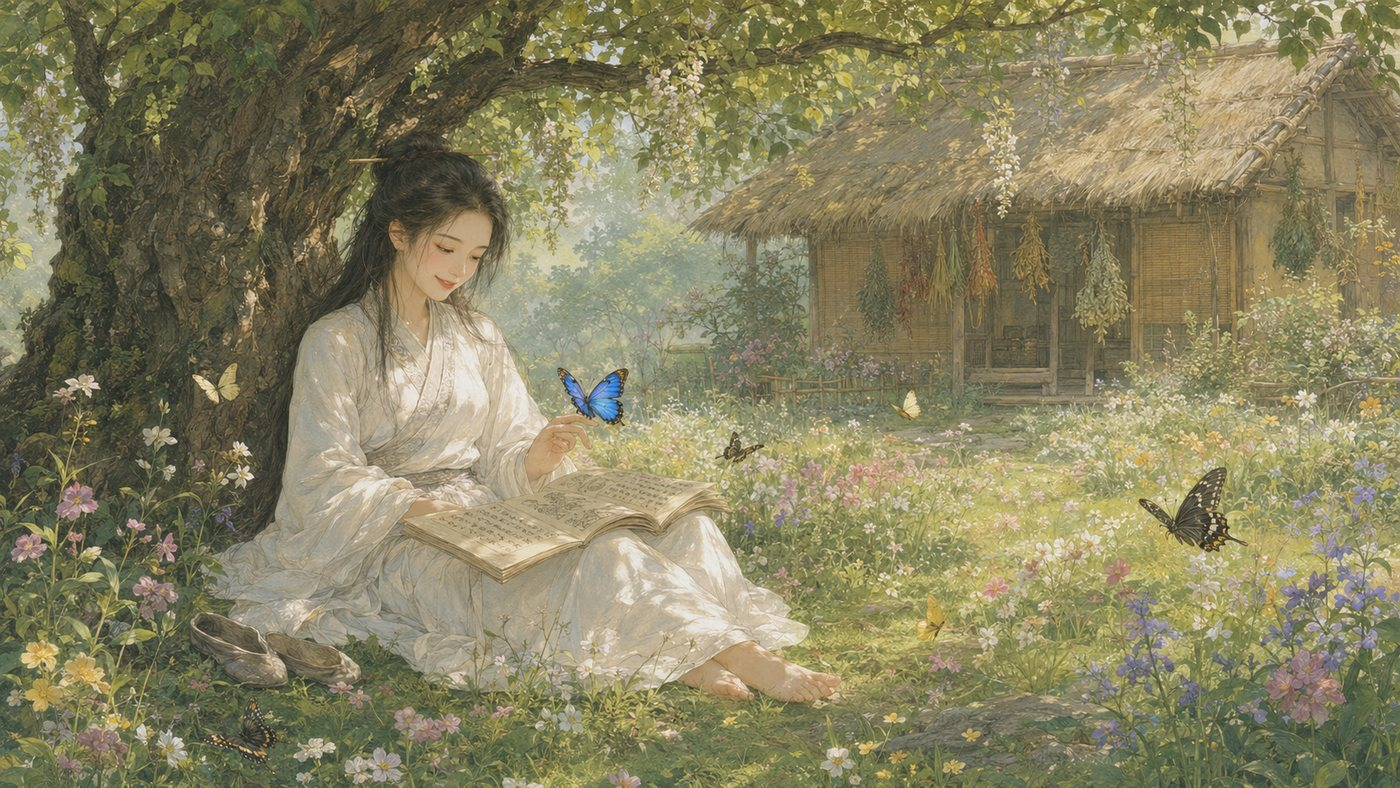
\includegraphics[width=0.92\linewidth,height=0.62\textheight,keepaspectratio]{assets/characters/zhaomin/portrait_12.jpg}
  \caption{赵敏第12拍《大都宫闱》人物图。大都宫闱。高墙、帷幕与狭窄天光表现权力空间的规训，人物目光越出画面，暗示精神上的出走。}
  \label{fig:portrait:zhaomin:12}
\end{figure}

\Needspace{0.72\textheight}
\begin{figure}[H]
  \centering
  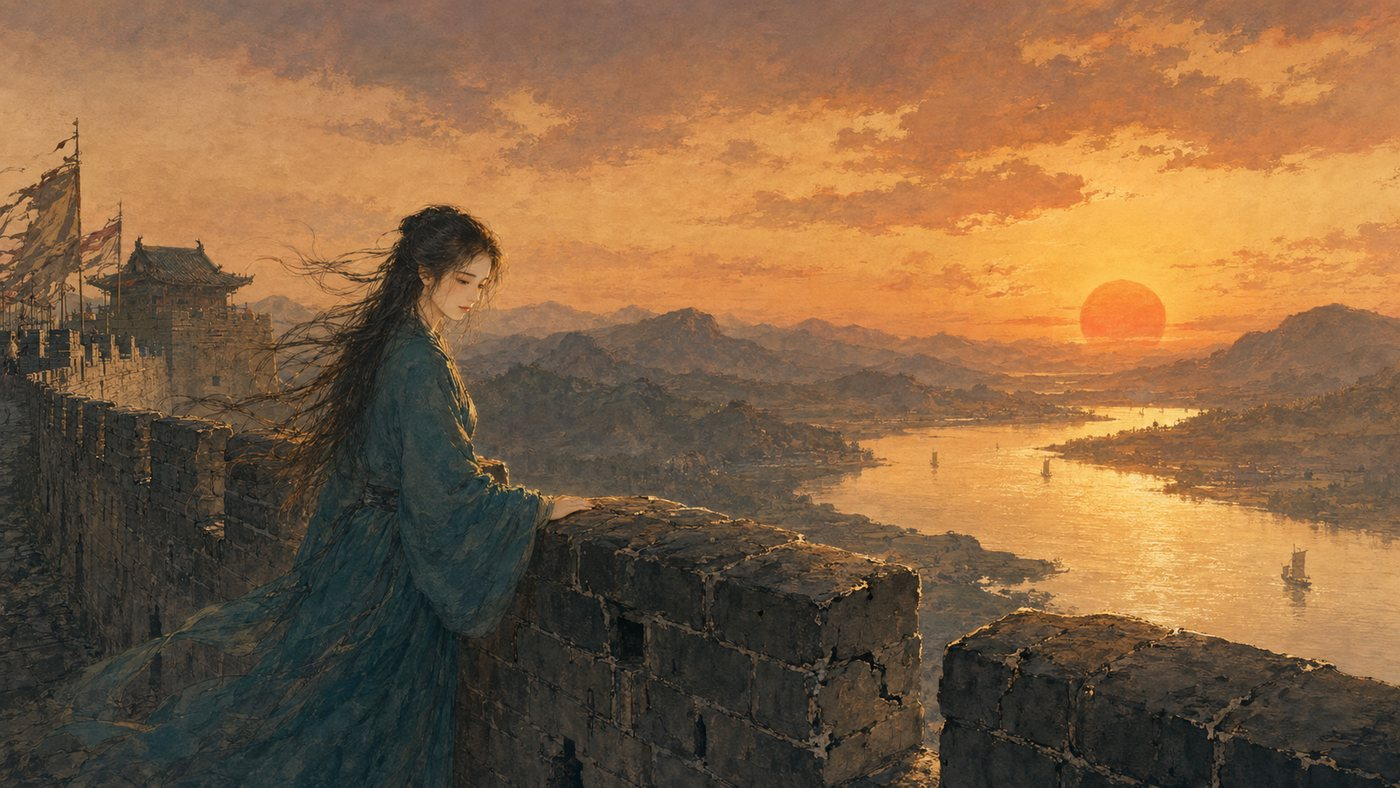
\includegraphics[width=0.92\linewidth,height=0.62\textheight,keepaspectratio]{assets/characters/zhaomin/portrait_13.jpg}
  \caption{赵敏第13拍《蝴蝶谷中》人物图。蝴蝶谷中。草木、药圃与缓和光线将照护置于日常劳动中；绿色层次表现医学知识与自然观察之间的联系。}
  \label{fig:portrait:zhaomin:13}
\end{figure}

\Needspace{0.72\textheight}
\begin{figure}[H]
  \centering
  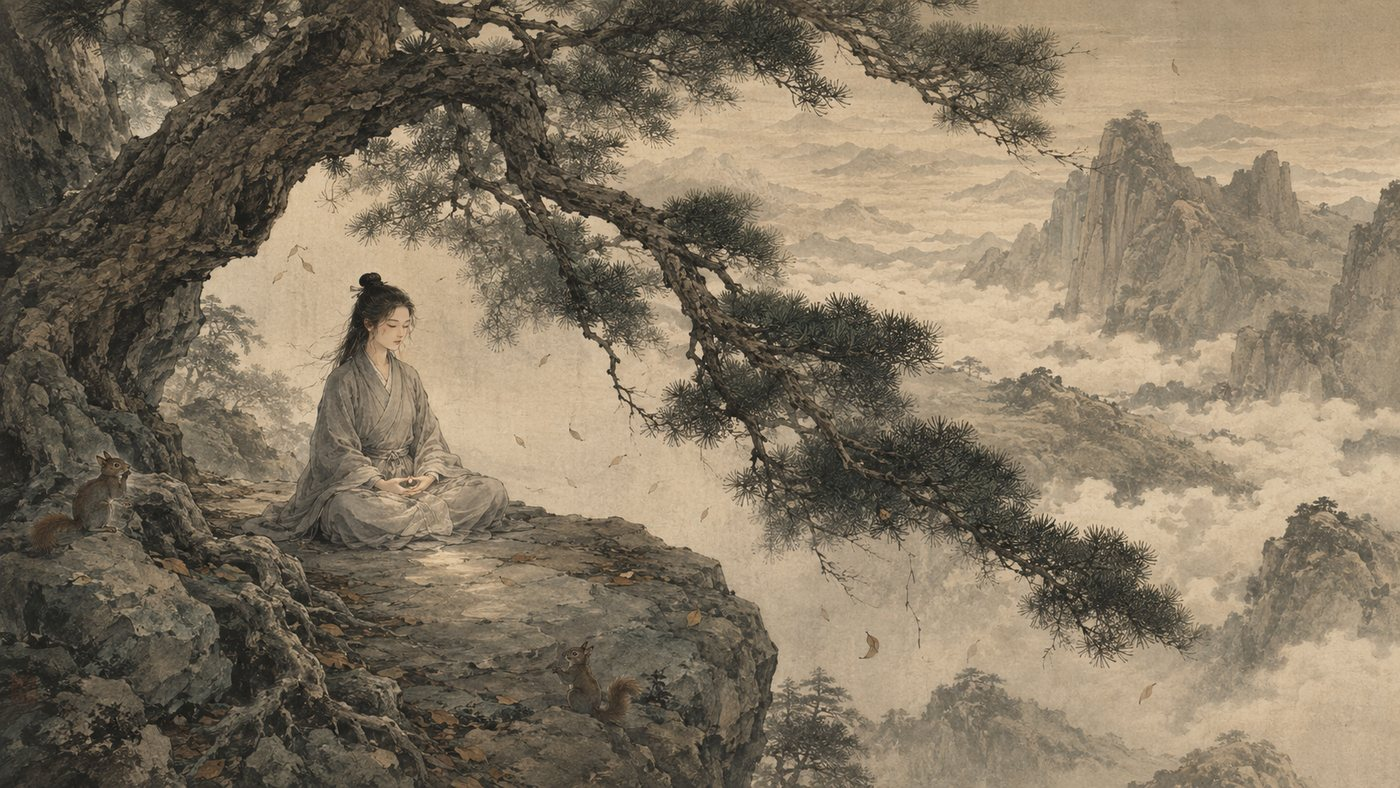
\includegraphics[width=0.92\linewidth,height=0.62\textheight,keepaspectratio]{assets/characters/zhaomin/portrait_14.jpg}
  \caption{赵敏第14拍《光明顶上》人物图。光明顶上。高山风云扩大人物行动的公共尺度，衣袂与云势同向，形成介入历史的动感；留白避免英雄化过度。}
  \label{fig:portrait:zhaomin:14}
\end{figure}

\Needspace{0.72\textheight}
\begin{figure}[H]
  \centering
  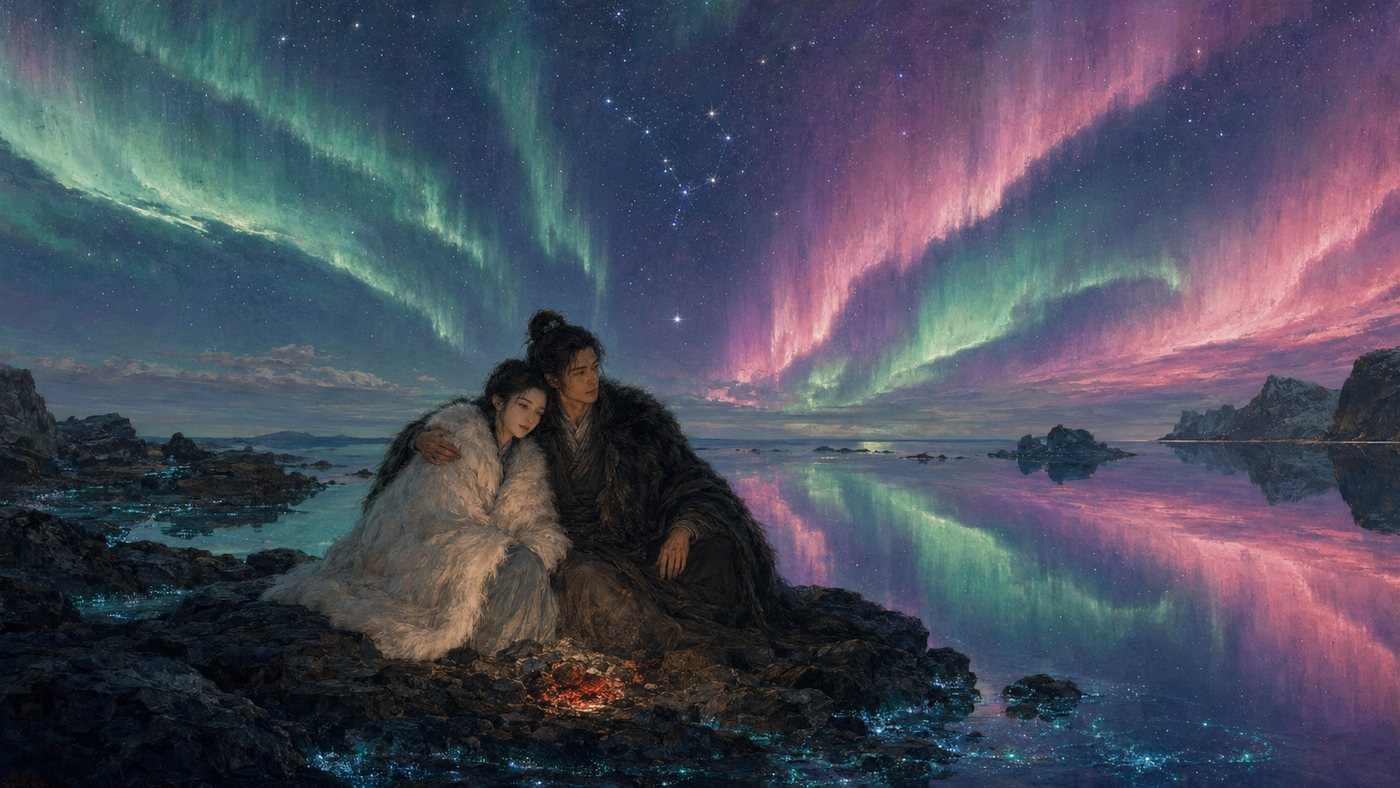
\includegraphics[width=0.92\linewidth,height=0.62\textheight,keepaspectratio]{assets/characters/zhaomin/portrait_15.jpg}
  \caption{赵敏第15拍《波斯异术》人物图。波斯异术。异域纹样与中原服饰并置，表现跨文化知识相遇；色彩差异被组织为互补关系，而非奇观化装饰。}
  \label{fig:portrait:zhaomin:15}
\end{figure}

\Needspace{0.72\textheight}
\begin{figure}[H]
  \centering
  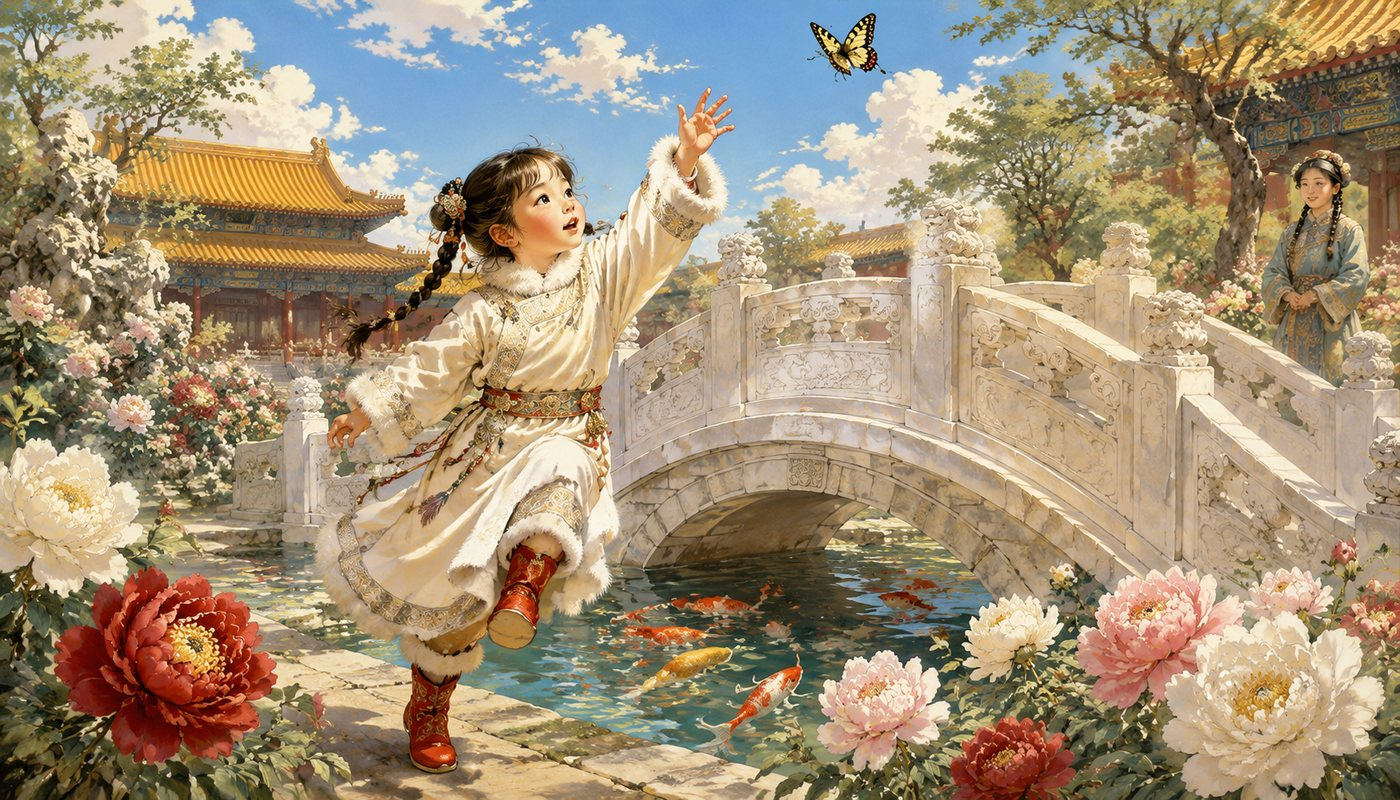
\includegraphics[width=0.92\linewidth,height=0.62\textheight,keepaspectratio]{assets/characters/zhaomin/portrait_16.jpg}
  \caption{赵敏第16拍《襄阳遗梦》人物图。襄阳遗梦。城墙、暮色与远方烽烟构成历史记忆，人物不再处于战斗中心；低饱和色调强调反思多于胜负。}
  \label{fig:portrait:zhaomin:16}
\end{figure}

\Needspace{0.72\textheight}
\begin{figure}[H]
  \centering
  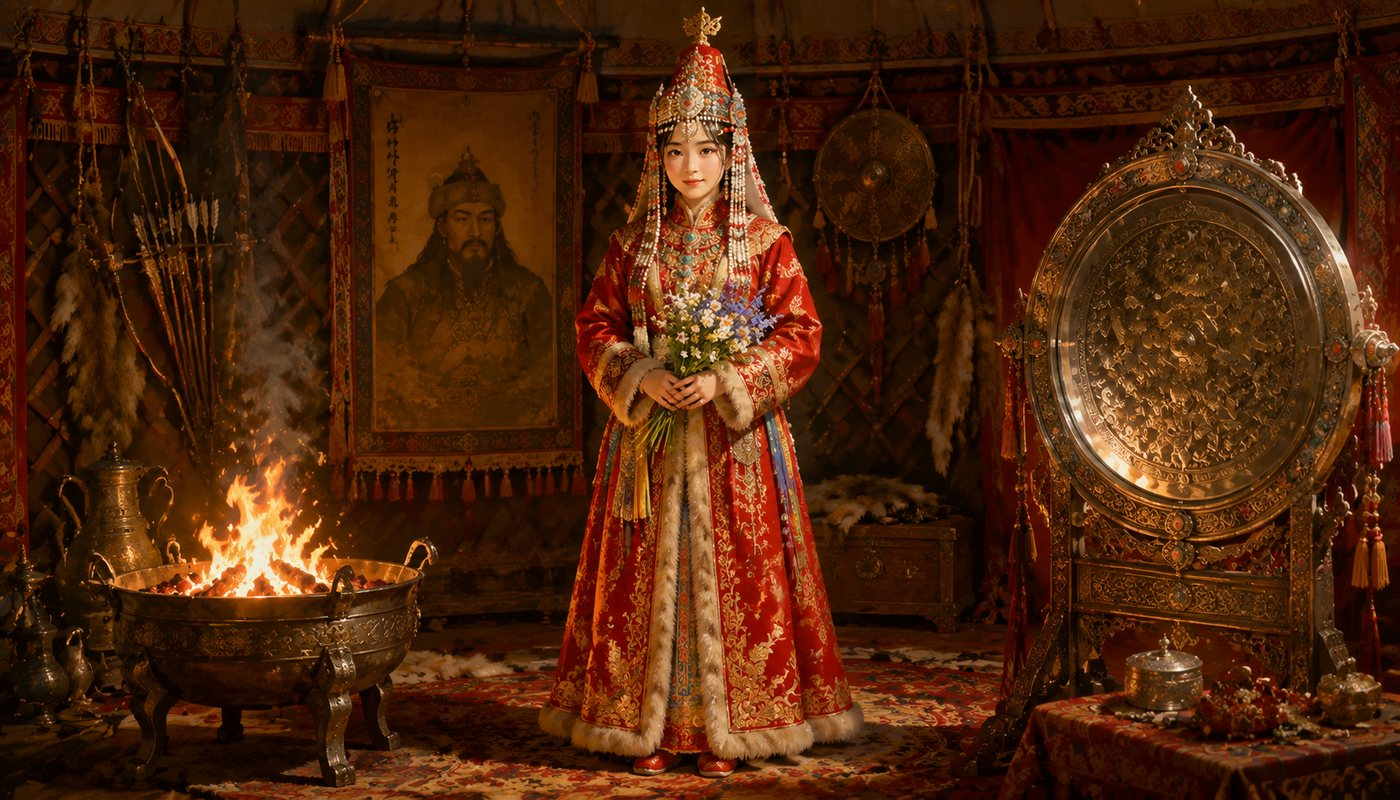
\includegraphics[width=0.92\linewidth,height=0.62\textheight,keepaspectratio]{assets/characters/zhaomin/portrait_17.jpg}
  \caption{赵敏第17拍《终南问道》人物图。终南问道。山径与云雾指向向内的追问，简化服饰和道具，削弱郡主身份；画面以清淡墨色表现精神减负。}
  \label{fig:portrait:zhaomin:17}
\end{figure}

\Needspace{0.72\textheight}
\begin{figure}[H]
  \centering
  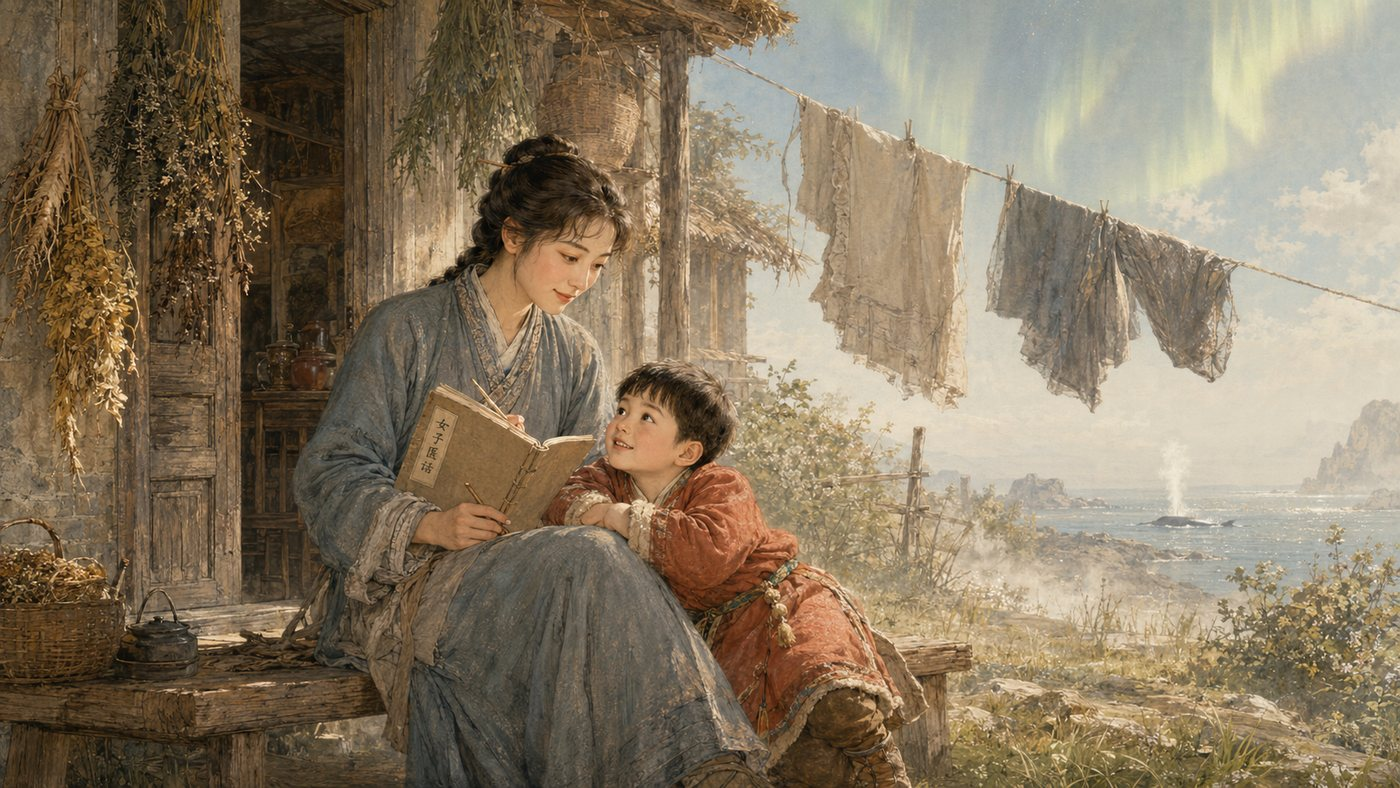
\includegraphics[width=0.92\linewidth,height=0.62\textheight,keepaspectratio]{assets/characters/zhaomin/portrait_18.jpg}
  \caption{赵敏第18拍《天下归心》人物图。天下归心。广阔天际与安定人间取代宫廷权力，人物神态平和；暖金色被控制在边缘光中，表达愿望而非凯旋。}
  \label{fig:portrait:zhaomin:18}
\end{figure}

\subsubsection{周芷若人物图录}

\Needspace{0.72\textheight}
\begin{figure}[H]
  \centering
  
\includegraphics[width=0.92\linewidth,height=0.62\textheight,keepaspectratio]{assets/characters/zhouzhiruo/portrait_01.jpg}
  \caption{周芷若第1拍《汉水初遇》人物图。汉水初遇。水岸、薄雾与少女形象建立生命早期的脆弱和澄明；低视点使人物与江流处于同一命运尺度。}
  \label{fig:portrait:zhouzhiruo:1}
\end{figure}

\Needspace{0.72\textheight}
\begin{figure}[H]
  \centering
  
\includegraphics[width=0.92\linewidth,height=0.62\textheight,keepaspectratio]{assets/characters/zhouzhiruo/portrait_02.jpg}
  \caption{周芷若第2拍《峨眉入门》人物图。峨眉入门。山门与规整石阶表现师门秩序，人物居于纵深入口，暗示成长始于接受也始于约束。}
  \label{fig:portrait:zhouzhiruo:2}
\end{figure}

\Needspace{0.72\textheight}
\begin{figure}[H]
  \centering
  
\includegraphics[width=0.92\linewidth,height=0.62\textheight,keepaspectratio]{assets/characters/zhouzhiruo/portrait_03.jpg}
  \caption{周芷若第3拍《光明一剑》人物图。光明一剑。剑势切开静态构图，表现命令、情感与身体动作之间的冲突；冷光强调决断所带来的创伤。}
  \label{fig:portrait:zhouzhiruo:3}
\end{figure}

\Needspace{0.72\textheight}
\begin{figure}[H]
  \centering
  
\includegraphics[width=0.92\linewidth,height=0.62\textheight,keepaspectratio]{assets/characters/zhouzhiruo/portrait_04.jpg}
  \caption{周芷若第4拍《万安寺誓》人物图。万安寺誓。高塔、夜色与微弱灯火构成封闭环境，人物姿态克制；竖向结构强化誓言的重量和不可退避感。}
  \label{fig:portrait:zhouzhiruo:4}
\end{figure}

\Needspace{0.72\textheight}
\begin{figure}[H]
  \centering
  
\includegraphics[width=0.92\linewidth,height=0.62\textheight,keepaspectratio]{assets/characters/zhouzhiruo/portrait_05.jpg}
  \caption{周芷若第5拍《灵蛇毒计》人物图。灵蛇毒计。海岛雾气遮蔽空间关系，象征猜疑与误认；人物与危险物之间保留距离，使伦理警觉先于戏剧刺激。}
  \label{fig:portrait:zhouzhiruo:5}
\end{figure}

\Needspace{0.72\textheight}
\begin{figure}[H]
  \centering
  
\includegraphics[width=0.92\linewidth,height=0.62\textheight,keepaspectratio]{assets/characters/zhouzhiruo/portrait_06.jpg}
  \caption{周芷若第6拍《裂裳之痛》人物图。裂裳之痛。破损衣料作为创伤痕迹而非猎奇细节，画面压低色彩与动作幅度，维护人物尊严。}
  \label{fig:portrait:zhouzhiruo:6}
\end{figure}

\Needspace{0.72\textheight}
\begin{figure}[H]
  \centering
  
\includegraphics[width=0.92\linewidth,height=0.62\textheight,keepaspectratio]{assets/characters/zhouzhiruo/portrait_07.jpg}
  \caption{周芷若第7拍《九阴白骨》人物图。九阴白骨。强烈墨色和骨白形成近乎失衡的视觉张力，表现力量对主体的反噬；边缘留白保存自我回返的可能。}
  \label{fig:portrait:zhouzhiruo:7}
\end{figure}

\Needspace{0.72\textheight}
\begin{figure}[H]
  \centering
  
\includegraphics[width=0.92\linewidth,height=0.62\textheight,keepaspectratio]{assets/characters/zhouzhiruo/portrait_08.jpg}
  \caption{周芷若第8拍《峨眉掌门》人物图。峨眉掌门。正面构图与门派器物呈现制度身份，人物目光略偏离中轴，提示权威与内心并未完全重合。}
  \label{fig:portrait:zhouzhiruo:8}
\end{figure}

\Needspace{0.72\textheight}
\begin{figure}[H]
  \centering
  
\includegraphics[width=0.92\linewidth,height=0.62\textheight,keepaspectratio]{assets/characters/zhouzhiruo/portrait_09.jpg}
  \caption{周芷若第9拍《屠狮之会》人物图。屠狮之会。群体空间被压缩为围合结构，表现公共审判的压力；人物处于视觉焦点，却不被塑造成单纯胜者。}
  \label{fig:portrait:zhouzhiruo:9}
\end{figure}

\Needspace{0.72\textheight}
\begin{figure}[H]
  \centering
  
\includegraphics[width=0.92\linewidth,height=0.62\textheight,keepaspectratio]{assets/characters/zhouzhiruo/portrait_10.jpg}
  \caption{周芷若第10拍《黄衫女子》人物图。黄衫女子。明黄与素白的相遇形成镜像关系，象征另一种女性力量介入；双主体构图避免把比较化为高下评判。}
  \label{fig:portrait:zhouzhiruo:10}
\end{figure}

\Needspace{0.72\textheight}
\begin{figure}[H]
  \centering
  
\includegraphics[width=0.92\linewidth,height=0.62\textheight,keepaspectratio]{assets/characters/zhouzhiruo/portrait_11.jpg}
  \caption{周芷若第11拍《问心有愧》人物图。问心有愧。空室、灯影与低垂视线将冲突转向内在，画面减少道具，让悔悟成为持续的伦理劳动。}
  \label{fig:portrait:zhouzhiruo:11}
\end{figure}

\Needspace{0.72\textheight}
\begin{figure}[H]
  \centering
  
\includegraphics[width=0.92\linewidth,height=0.62\textheight,keepaspectratio]{assets/characters/zhouzhiruo/portrait_12.jpg}
  \caption{周芷若第12拍《汉水归舟》人物图。汉水归舟。归舟重返最初的水域意象，江面留白承接记忆与宽恕；人物背影弱化身份标签，突出返身自省。}
  \label{fig:portrait:zhouzhiruo:12}
\end{figure}

\Needspace{0.72\textheight}
\begin{figure}[H]
  \centering
  
\includegraphics[width=0.92\linewidth,height=0.62\textheight,keepaspectratio]{assets/characters/zhouzhiruo/portrait_13.jpg}
  \caption{周芷若第13拍《峨眉金顶》人物图。峨眉金顶。云海与金顶构成超越性背景，人物尺度被有意缩小；宏阔空间不再服务权威，而用于重新理解归属。}
  \label{fig:portrait:zhouzhiruo:13}
\end{figure}

\Needspace{0.72\textheight}
\begin{figure}[H]
  \centering
  
\includegraphics[width=0.92\linewidth,height=0.62\textheight,keepaspectratio]{assets/characters/zhouzhiruo/portrait_14.jpg}
  \caption{周芷若第14拍《药王谷中》人物图。药王谷中。药架、草木与书写活动表现知识由秘术转向公共照护；柔和自然光建立可学习、可传承的医学氛围。}
  \label{fig:portrait:zhouzhiruo:14}
\end{figure}

\Needspace{0.72\textheight}
\begin{figure}[H]
  \centering
  
\includegraphics[width=0.92\linewidth,height=0.62\textheight,keepaspectratio]{assets/characters/zhouzhiruo/portrait_15.jpg}
  \caption{周芷若第15拍《襄阳城墙》人物图。襄阳城墙。城垣与远山并置个人创伤和共同历史，人物站姿稳定而不昂扬；沉着色调表达守护而非征服。}
  \label{fig:portrait:zhouzhiruo:15}
\end{figure}

\Needspace{0.72\textheight}
\begin{figure}[H]
  \centering
  
\includegraphics[width=0.92\linewidth,height=0.62\textheight,keepaspectratio]{assets/characters/zhouzhiruo/portrait_16.jpg}
  \caption{周芷若第16拍《终南古墓》人物图。终南古墓。幽暗石室与出口微光形成生命转折，人物向光而行；空间叙事把挣脱执念转译为可见路径。}
  \label{fig:portrait:zhouzhiruo:16}
\end{figure}

\Needspace{0.72\textheight}
\begin{figure}[H]
  \centering
  
\includegraphics[width=0.92\linewidth,height=0.62\textheight,keepaspectratio]{assets/characters/zhouzhiruo/portrait_17.jpg}
  \caption{周芷若第17拍《华山论剑》人物图。华山论剑。高峰风势和开阔远景保留武侠传统，却让人物收剑而立；不出招的姿态象征力量获得节制。}
  \label{fig:portrait:zhouzhiruo:17}
\end{figure}

\Needspace{0.72\textheight}
\begin{figure}[H]
  \centering
  
\includegraphics[width=0.92\linewidth,height=0.62\textheight,keepaspectratio]{assets/characters/zhouzhiruo/portrait_18.jpg}
  \caption{周芷若第18拍《白莲重生》人物图。白莲重生。莲花从含苞、盛放到结蓬呈现完整生命循环，赤足掬水使身体重新接触自然；麻衣、晨光与水纹共同表达朴素的新生。}
  \label{fig:portrait:zhouzhiruo:18}
\end{figure}
